Pour diriger et faciliter l'évolution du projet, un certain nombre d'outils et de méthodes ont été mis en place au début du projet.
L'environnement avait pour but de permettre un développement agile. 
On peut distinguer 3 parties, la gestion du projet, la gestion des sources et les outils de développements.
\section{Planification et gestion de projet}
La méthode agile préconise des itérations courtes avec des objectifs clairs et concis à réaliser à chaque itération.
A chaque itération, un point est fait avec le client pour définir les objectifs pour la prochaine itération, le client ici étant notre tuteur, Julien Ponge.
Nous avons utilisé un outil pour gérer ces objectifs et ces itérations. Il s'agit est LightHouse.
\subsection{Lighthouse}
Lighthouse est un gestionnaire de projet en ligne.
Il se présente sous la forme d'une application web et propose toutes les fonctionnalités nécessaires à la gestions des objectifs.
On peut distinguer deux entités principales, les tickets et les sprints.
\begin{figure}[H]
	\centering
	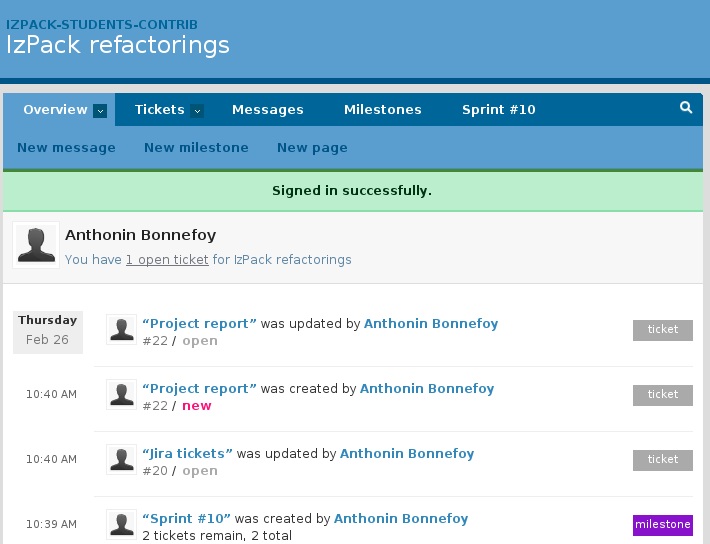
\includegraphics[width=0.4\textwidth]{../image/lighthouse.png}
	\caption{Page d'accueil de Lighthouse}
\end{figure}
\subsection{Ticket}
Les Tickets représentent un objectif à réaliser.
Ils peuvent être crées par n'importe quel participant au projet. 
Ce ticket peut ensuite être assigner à une personne et possède plusieurs états.
\begin{itemize}
\item Nouveau
\item Ouvert
\item Résolu
\item Clos
\end{itemize}

Chacun de ces tickets peut être assigné à un sprint.
\subsection{Sprint}
Un sprint est un ensemble de tickets à résoudre pour une date donnée. 
Il correspond à une itération dans la méthodologie agile.
Pour le projet, la durée d'un sprint était généralement de 1 ou 2 semaines.
A chaque fin de sprint, une réunion était organisée pour discuter des résultats, des reports à effectuer ou des objectifs à réaliser pour le prochains sprint.
\section{Gestionnaire des sources}
\subsection{Gestionnaire de versions}
Tout projet informatique conséquent se doit d'être sous gestionnaire de version.
En effet, un gestionnaire de version permet de suivre l'évolution du code source dans le temps.
Un dépôt conserve l'historique des changements ce qui permet de revenir à une version antérieur.
De plus, il facilite le travail collaboratif.
En effet, les développeurs travaillant de manière indépendante sur leur version du programme, la mise en commun est prise en charge par le gestionnaire.
Il permet alors de résoudre les conflits et de fusionner les fichiers modifiés.

Izpack étant un projet open-source actif, de nombreuses modifications étaient appliquées régulièrement.
Il fallait donc pouvoir travailler en parallèle des changements opérés par les contributeurs et pouvoir appliquer facilement nos modifications le jour venu.

Le dépôt de référence d'IzPack est un dépôt Subversion.
Les contributeurs appliquent leurs modifications sur ce dépôt.
Cependant, pour des raisons de facilité et pour ne pas perturber le développement, il a été décidé de travailler sur un fork Git plutôt que sur le dépôt subversion.
\subsection{Git}
Git est un gestionnaire de version récent. Il a été crée en 2004 par Linus Torvald pour remplacer BitKeeper, l'ancien gestionnaire de version du noyau linux.
Il s'agit, à l'instar de BitKeeper, d'un système distribué.
Toutes les copies du dépôt sont elles-mêmes des serveurs.
Chaque personne travaille donc sur son propre dépôt et se synchronise par rapport à d'autres dépôts.
C'est de cet aspect distribué que provient une grande partie de la puissance de Git.
Un utilisateur a accès à l'historique entier une fois qu'il a cloné le dépôt.
Il peut effectuer toutes les operations voulues sur son dépôt en étant déconnecté et chaque clone est une sauvegarde intégrale du dépôt.
Ainsi, n'importe quel développeur a accès à toutes les fonctionnalités d'un gestionnaire de version même s'il n'est pas connecté au dépôt central.
La communication entre dépôts Git se fait soit par le protocole ssh, https, ftp, rsync ou par le protocole git.

Git se démarque également sur des fonctionnalités évoluées. 
L'un de ses principaux points forts est la gestion des branches. 
La création, suppression et fusion des branches est remarquable de simplicité et d'efficacité.
La taille d'un dépôt Git est faible comparée à celle d'autres gestionnaires comme subversion.

Julien Ponge entretient un dépôt Git synchronisé par rapport au Subversion. 
Nous avons travaillé sur un fork de ce dépôt.
Nous pouvions à tout moment synchroniser notre dépôt par rapport au dépôt d'origine et ainsi, appliquer toutes les modifications des contributeurs à notre dépôt.
Cela permettait de préparer l'application de nos modifications de manière aisée. Tout ces dépôts sont hébergés sur GitHub.
\subsection{GitHub}
GitHub est une plateforme collaborative hébergeant des dépôts Git. 
Cette plateforme permet de créer, dupliquer, supprimer ou consulter des dépôts Git.
Toutes les réalisations faites sont ouvertes et disponibles à tout le monde, c'est à dire que n'importe qui est libre de consulter, cloner ou de forker les projets présents sur GitHub.
Le droit de commit est cependant restreint aux utilisateurs choisies.
Cette plateforme a été choisi par Julien Ponge pour héberger son dépôt Git. 
Nous nous sommes donc créés des comptes sur GitHub et l'avons forké. 
L'utilisation d'un dépôt public basé sur celui de Julien Ponge a permis non seulement de faciliter les mises à jour, mais également de lui permettre de suivre facilement notre travail.
%- GitHub : Gestionnaire de dépôt Git
%-> Duplicat (fork) du projet
%-> Travail collaboratif et ouvert 
%-> Consultation de l'historique
%-> Visionnage des branches
\section{Outils de développement}
\subsection{IntelliJ Idea}
%-> IDE spécialisée technologies Java
%Nombreuses fonctionnalités présentes
%-> Recherche implementation 
%-> Preserve Case
%-> Refactoring puissant
IntelliJ est un environnement de développement intégré similaire à Eclipse.
Il est propriétaire et nécessite une licence pour son fonctionnement. 
Cependant, JetBrain, l'éditeur de IntelliJ, a une politique d'ouverture pour les projets open-source.
Les projets sous CodeHaus et Apache bénéficient d'une licence dédiée et gratuite. 

Il présente certaines divergences avec des IDE comme Eclipse et NetBeans.
Il possède une plus grande variété de fonctionnalités et l'intégration d'un grand nombre de composants.
On trouve ainsi l'intégration de frameworks récents comme GWT ou d'outils comme Git.
L'intégration de Maven est également très complète.
De plus, ses capacités de modification de code (refactoring) sont au dessus de celles des autres IDE : préservation de la casse lors d'un renommage, etc.
\subsection{Yourkit}
%Profiler Java
%-> Temps, nombres d'appels des méthodes
%-> Affichage de la charge a tout moment
Yourkit est un outil de profiling. Il permet d'avoir un rapport détaillé sur l'utilisation des ressources par le programmes. On peut ainsi récupérer le nombre d'appel à une méthode, le temps passé dans une méthode, l'utilisation des ressources à un temps donné.

Le but du profiling a été de repérer les optimisations possibles sur les modifications que l'on a opérées.
%TODO Faire des snapshots yourkit